%%%%%%%%%%%%%%%%%%%%%%%%%%%%%%%%%%%%%%%%%%%%%%
%                insertmeeting
% 1) Title (something creative & funny?)
% 2) Date (MM/DD/YYYY)
% 3) Location (ex. Hagerty High School)
% 4) People/Committees Present 
% 5) Picture 
% 6) Start Time & Stop Time (ex. 12:30AM to 4:30PM)
%%%%%%%%%%%%%%%%%%%%%%%%%%%%%%%%%%%%%%%%%%%%%%
\insertmeeting 
	{I Didn't Know I Was Lost} 
	{03/22/22} 
	{Hagerty High School}
	{James, Jensen, Nathan, Ritam}
	{Images/RobotPics/robot.jpg}
	{2:30 - 4:30}
	
\hhscommittee{Software}
\noindent\hfil\rule{\textwidth}{.4pt}\hfil
\subsubsection*{Goals}
\begin{itemize}
    \item Explore the pros and cons of Ramsete and PIDVA controllers

\end{itemize} 

\noindent\hfil\rule{\textwidth}{.4pt}\hfil

\subsubsection*{Accomplishments}
In the Road Runner library that we are using, there are multiple options for the mathematical controller to use. The most popular option is the Ramsete controller. While many of the articles on the Internet were filled with advanced math and complicated terminology, we just decided to treat it as a black box, since the implementation was already present. Essentially, it is a feedback controller similar to PID that is designed specifically for differential drives, extremely similar to our tricycle drivetrain. On the other hand, the PIDVA follower was just a normal PID controller with feedforward constants for the velocity and acceleration, slightly improving performance. When we switched between the two, there was not a huge difference. Both controllers did well, moving the robot according to the trajectories laid out. However, one thing we did notice was that the PIDVA controller resulted in slightly more oscillation when tracking the trajectories drawn on the graph from FTC Dashboard. As a result, we decided to continue using the Ramsete controller. 


\begin{figure}[htp]
\centering
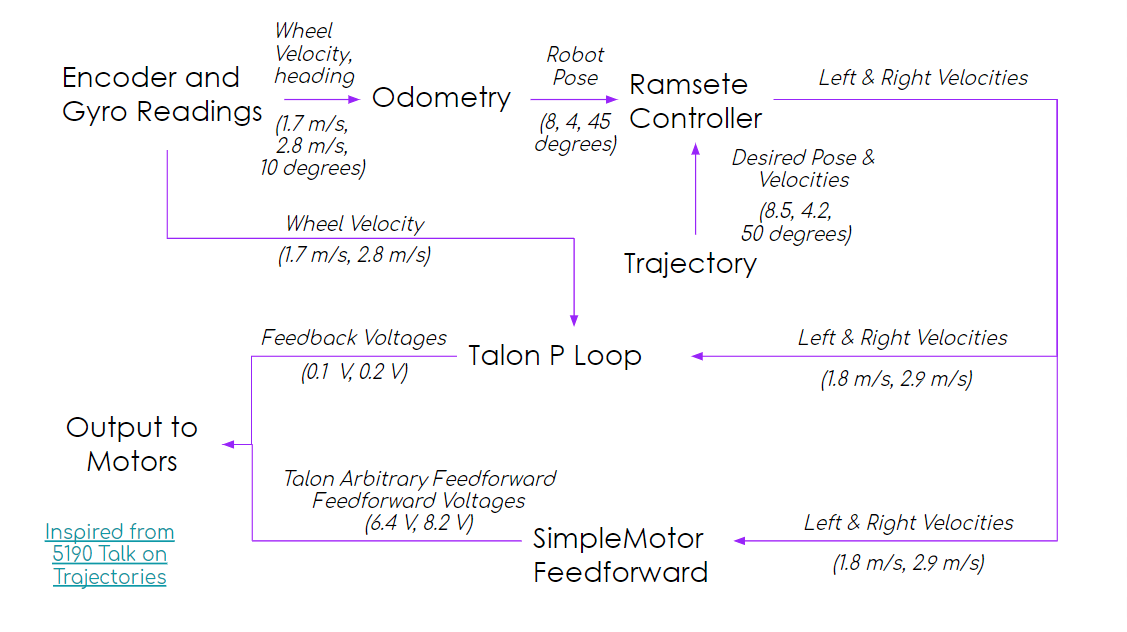
\includegraphics[width=0.95\textwidth, angle=0]{Meetings/March/03-22-22/03-22-22 1.png}
\caption{An infographic summarizing the Ramsete controller from FRC5190.}
\label{fig:032222_1}
\end{figure}



\whatsnext{
\begin{itemize}
    \item Add more cycles to the autonomous programs. 
\end{itemize} 
}

